\documentclass[a4paper]{article}
\setlength\parindent{1.5em}

\usepackage{indentfirst}
\usepackage[utf8]{inputenc}
\usepackage[T1]{fontenc}
\usepackage{textcomp}
\usepackage[russian]{babel}
\usepackage{amsmath, amssymb}
\usepackage{graphicx }

% figure support
\usepackage{import}
\usepackage{xifthen}
\pdfminorversion=7
\usepackage{pdfpages}
\usepackage{transparent}
\newcommand{\incfig}[1]{%
  \def\svgwidth{\columnwidth}
  \import{./figures/}{#1.pdf_tex}
}

\pdfsuppresswarningpagegroup=1
\title{Информатика}
\author{Ситников Михаил}
\date{\today}

\begin{document}
\maketitle
\section{Введение}
\subsection{КФС. Основные свойства. БТС.}
\begin{figure}[htpb]
  \centering
  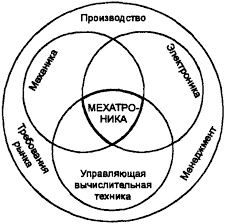
\includegraphics[width=0.8\textwidth]{figures/mechatronics.png}
  \caption{}
  \label{fig:}
\end{figure}
\paragraph{Определения}
\par
Киберр-физическая система интегриркет способности к вычислениям, связи и хранению информации с мониторингом и управлением объектами физического мира и должна делать это надежно, безопасно, эффективно и в реальном времени. Киьбер-физические системы должны быть расширяемыми, экономичными и адаптивными.
\par
Информамционно-технологическая концепция, подразумевающая интерграцию вычислительных ресурсов в физические сущности любого вида, включая биологические и рукотворные объекты.
\paragraph{История робототехники}
\begin{itemize}
  \item Движущиеся статуи (I век до нашей эры)
  \item Механические устройства (Леонардо да Винчи)
  \item Автоматоны
  \item Разностная машина
  \item Boilerplate 
\end{itemize}
\paragraph{Промышленные работы}
\begin{itemize}
  \item Манипуляторы 
  \item John Hopkins Beast (1960)
  \item Shakey (1970)
  \item Луноход
  \item Марсоход
\end{itemize}
\paragrah{Тенденции развития}
\begin{itemize}
  \itemРазработка стандартов
  \itemУменьшение размеров
  \itemУдешевение стоимости комплектующих
  \itemРазвитие систем управления
  \begin{itemize}
    \itemИИ
    \itemСтайное управление
    \itemФункционирование в условиях неопределенности
  \end{itemize}
\end{itemize}
\paragraph{Список литературы}
\begin{itemize}
  \item
\end{itemize}

\paragraph{Состояния системы}
\begin{center}
$E = E^{uf} \cup E^{pby}$
\par
$S_e = f(E, U)$
\par
$U = U_{out} \cup U_{in}$
\par
Внешнее воздействие
\par
$\frac{dS}{dt}= F(E^t, U^t)$

\end{center}
\par
U -- вход
\par
Y -- выход
\par
$|Y| = |U|$ 
\par
$Y^{-1} = U$

\paragraph{Виды архитектур интелектуальных агентов}
\begin{itemize}
  \itemРеактивный
  \itemДелиберативный
\end{itemize}
\paragraph{Цели для беспилотников}
\begin{enumerate}
  \itemСтабилизация
  \par
  $y(t) \to y^x$ 
  \par$\lim |u^x - y(t)| \le \nu$
  \itemСложение
  \itemВозбуждение (разгон)
  \itemСинхронность
\end{enumerate}
\end{document}
